\chapter{Testing}
\label{chap:results}

A partner work implemented a method to calculate the gaze direction with two fitted ellipses from different cameras of the same eye. Together with the algorithm described in the last chapter, it is possible to calculate the gaze direction from picture data. Results from both eyes are intelligently combined to improve the accuracy. More information about how this is accomplished can be found in the partner work\cite{bleuer}. The pictures and parameters generated in chapter \ref{chap:Model} can now be used to compare the result of the algorithms with the parameters.

\subsubsection{Animation}
\label{sec:animation}

The animation for this test should cover a wide variety of gaze directions. Otherwise, directions that produce strange results could be missed. Additionally, no big jumps should occur as the algorithm for the pupil detection uses the last frame as reference.

A path that fulfils those requirements is shown in figure \ref{fig:path}. It covers a wide area of 40$^{\circ}$ in all directions and follows the path with a steady speed.

\begin{figure} [H]
	\centering
	\includegraphics[width=0.4\linewidth]{images/grid.png}
	\caption{Path that the eyes follow during the animation. It starts at \{-20$^{\circ}$, -20$^{\circ}$\} and follows the black in a horizontal zick-zack pattern path until it reaches \{20$^{\circ}$, 20$^{\circ}$\}. From there it follows the blue vertical zick-zack pattern path until it reaches the start point again. }
	\label{fig:path}	
\end{figure}

You would expect a higher resolution to produce a more accurate result. The animation was rendered at \gls{QVGA}(240x320), \gls{VGA}(480x640) and \gls{UVGA}(960x1280) resolutions to test that hypothesis. 
\subsubsection{Results}

The fixed threshold algorithm and the filter algorithm were both applied to every resolution. The result for the \gls{VGA} resolution with fixed and filter algorithm are presented in figure \ref{fig:VGA}. It seems that the filter algorithm performs worse than the fixed threshold algorithm. This is confirmed by a look at the standard deviation. The filter algorithm performs much worse at the lower \gls{VGA} and \gls{QVGA} resolutions as shown in figure \ref{fig:fixedMiddle}. A big contribution to this discrepancy is much higher maximal deviation. 

\begin{figure}
	\begin{subfigure}{.5\textwidth}
		\centering
		\includegraphics[width=\linewidth]{images/fixed_middle.png}
		\caption{Fixed Algorithm}
		\label{fig:fixedMiddle}
	\end{subfigure}
	\begin{subfigure}{.5\textwidth}
		\centering
		\includegraphics[width=\linewidth]{images/normal_middle.png}
		\caption{Filtered Algorithm}
		\label{fig:normalMiddle}
	\end{subfigure}

	\caption{Comparison between the gaze direction obtained by the log of the animation(dashed) and calculated direction with the algorithms(solid). The results for the fixed threshold in figure \ref{fig:fixedMiddle} seem more accurate than the results for the filter algorithm in figure \ref{fig:normalMiddle}.}
	\label{fig:VGA}
\end{figure}

\begin{figure}
\begin{subfigure}{.5\textwidth}
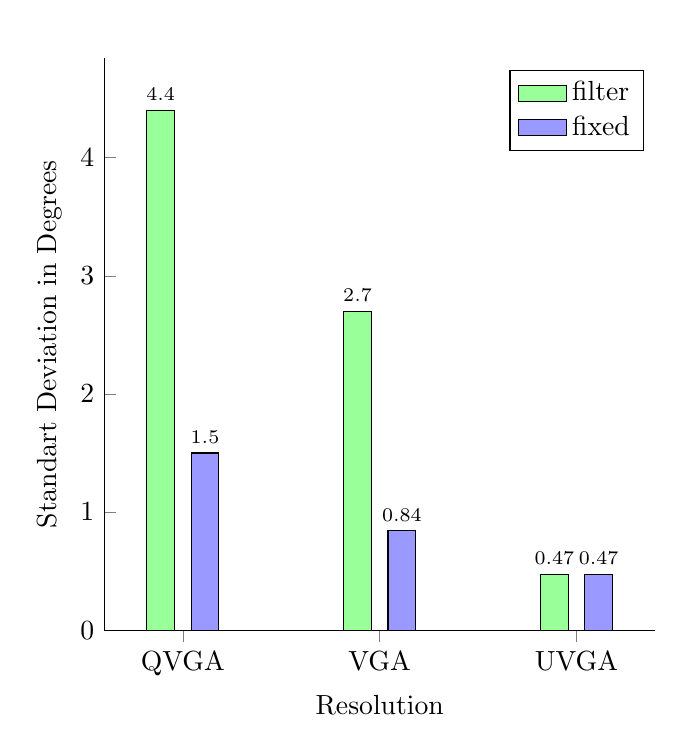
\begin{tikzpicture}
\begin{axis}[
%legend columns=-1,
legend cell align=left,
every axis plot post/.style={/pgf/number format/fixed},
ybar=6pt,
bar width=10pt,
x=2.5cm,
y=1.5cm,
ymin=0,
axis on top,
%ymax=12,
xtick=data,
%xlabel=Cores,
ylabel=Standart Deviation in Degrees,
xlabel=Resolution,
enlarge x limits=0.2,
%enlarge y limits={abs=0.5},
symbolic x coords={QVGA,VGA,UVGA},
%restrict y to domain*=0:11, % Cut values off at 14
visualization depends on=rawy\as\rawy, % Save the unclipped values
after end axis/.code={ % Draw line indicating break
	\draw [ultra thick, white] (rel axis cs:0,1.05) -- (rel axis cs:1,1.05);
},
nodes near coords={\scriptsize{\pgfmathprintnumber{\rawy}}
},
axis lines*=left,
clip=false,
area legend
%legend style={at={(0.6,0.8)},anchor=west}
]
\addplot[fill=green!40] coordinates {(QVGA,4.4) (VGA,2.7) (UVGA,0.47) };
\addplot[fill=blue!40] coordinates {(QVGA,1.5) (VGA,0.84) (UVGA,0.47)};
\legend{filter,fixed};
\end{axis}
\end{tikzpicture}
\caption{}
\label{fig:standartDeviation}
\end{subfigure}
\begin{subfigure}{.5\textwidth}
	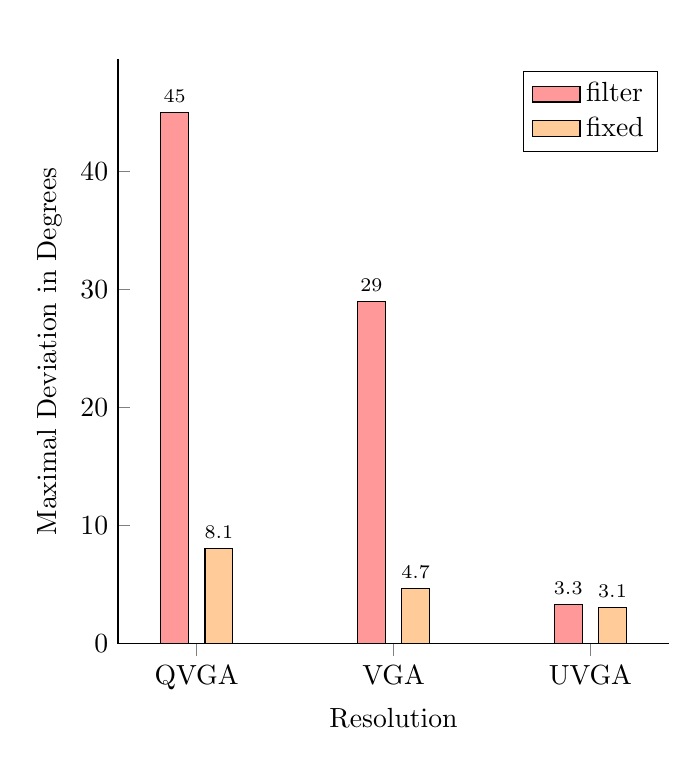
\begin{tikzpicture}
	\begin{axis}[
	%legend columns=-1,
	legend cell align=left,
	every axis plot post/.style={/pgf/number format/fixed},
	ybar=6pt,
	bar width=10pt,
	x=2.5cm,
	y=0.15cm,
	ymin=0,
	axis on top,
	%ymax=12,
	xtick=data,
	%xlabel=Cores,
	ylabel=Maximal Deviation in Degrees,
	xlabel=Resolution,
	enlarge x limits=0.2,
	%enlarge y limits={abs=0.5},
	symbolic x coords={QVGA,VGA,UVGA},
	%restrict y to domain*=0:11, % Cut values off at 14
	visualization depends on=rawy\as\rawy, % Save the unclipped values
	after end axis/.code={ % Draw line indicating break
		\draw [ultra thick, white] (rel axis cs:0,1.05) -- (rel axis cs:1,1.05);
	},
	nodes near coords={\scriptsize{\pgfmathprintnumber{\rawy}}
	},
	axis lines*=left,
	clip=false,
	area legend
	%legend style={at={(0.6,0.8)},anchor=west}
	]
	\addplot[fill=red!40] coordinates {(QVGA,45) (VGA,29) (UVGA, 3.3) };
	\addplot[fill=orange!40] coordinates {(QVGA,8.1) (VGA,4.7) (UVGA,3.1)};
	\legend{filter,fixed};
	\end{axis}
	\end{tikzpicture}
	\caption{}
	\label{fig:maximalDeviation}
\end{subfigure}
\caption{Figure \ref{fig:standartDeviation} shows the standart deviation between the resolutions and different algorithm. The filter algorithm performs similar to the fixed threshold algorithm at the \gls{UVGA} resolution. But at the lower resolutions it performs much worse. An explanation for that can be found in the maximal deviation in Figure \ref{fig:maximalDeviation}. The maximal deviation is much bigger for the filter algorithm.}
\label{fixedVsFilter}
\end{figure}
\subsubsection{Discussion}
It is quite surprising how much better the fixed threshold algorithm performs at the lower resolutions. It has to be noted that the measurements are not with real data. Once the algorithm is implemented on GazelleCompute, measurements with actual data should be done.

Initially it was planed to configure the cameras with \gls{QVGA} resolution and a frame rate of 120fps. The results presented in figure \ref{fig:standartDeviation} show a reduction of the standard deviation of 44\% for the fixed threshold algorithm. This is an improvement that strongly favors the VGA resolution. For the Gazelle project the higher resolution would come at the cost of a reduced frame rate of 90fps instead of the planned 120.